\section{Experimental results}
\label{sec:experimental_results}
In this section, we present experimental results of a sensor analytics application for SHM and its hardware deployment.

To demonstrate the HF6 quantization, we implement an analytics application to predict x- y- coordinates of structural anomalies based on acoustic sensor data with CNN-regression models. We address the model design exploration using TensorFlow and Keras library.

To demonstrate the HF6 hardware concept, we deploy the CNN model for low-power inference in the smallest Zynq SoC. For comparison, the hardware engine is implemented with 32-bit floating-point, 8-bit fixed-point, and HF6. We address the hardware design exploration using HLS.

We present statistical evaluations of the CNN models with standard floating-point, fixed-point, and HF6 quantization. We evaluate the computational latency, resource utilization, and power dissipation. Finally, we present a discussion of the presented results.

\subsection{CNN Model Design Exploration}

\begin{figure*}[t!]
	\centering
	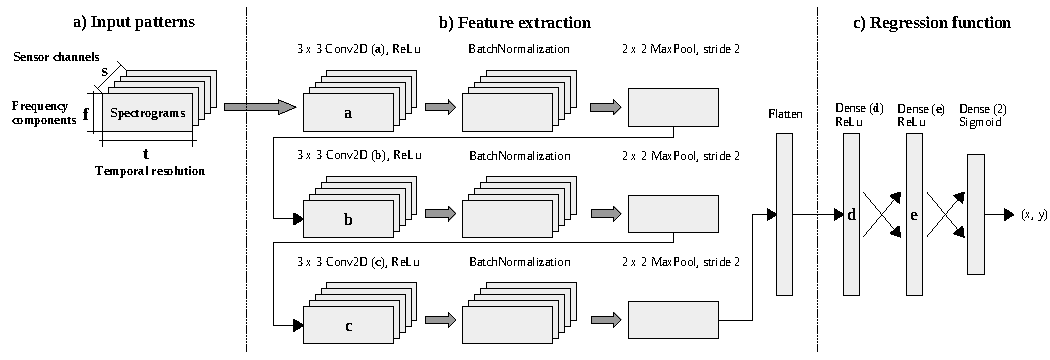
\includegraphics[width=\textwidth]{../figures/model.pdf}
	\caption{CNN model for case study.}
	\label{fig:models}
\end{figure*}

\subsection{Hardware Design Exploration}
The proposed hardware/software co-design framework is demonstrated on the MiniZed development board with a Zynq-7007S system-on-chip (SoC). This device integrates a single ARM Cortex-A9 processing system (PS) and programmable logic (PL) equivalent to Xilinx Artix-7 (FPGA) in a single chip \cite{xilinx2015zynq}. The Zynq-7007S SoC architecture maps the custom logic and software in the PL and PS respectively as an embedded system.

In this platform, we implement the proposed hardware architecture to deploy the \REVIEWR{CNN model} for \REVIEWR{SHM} shown in \Fig{fig:models}. The CNN model is created, trained, and quantized using Keras/TensorFlow with Python on a desktop computer. The resulting model is converted to TensorFlow Lite, which is deployed on the MiniZed. The Zynq-7007S SoC performs the model inference with TensorFlow Lite core API running on the PS. The computational workload of the convolution layers is delegated to the TP on the PL.

\subsection{Performance benchmark}
\subsubsection{Benchmark on embedded CPU}

We examine the performance of the embedded CPU for inference with no hardware acceleration. In this case, the embedded software builds the CNN as a sequential model mapping the entire computation to the CPU (ARM Cortex-A9) at 666 MHz and a power dissipation of \REVIEWR{$1.658 W$}.

The inference on the CPU achieves a latency of \REVIEWR{$40 ms$}. The model is computed with standard floating-point arithmetic with no accuracy degradation. The latency and schedule of the CNN inference are displayed in \Tab{tab:latency_sw} and \fig{fig:latency_sw} respectively.

\begin{table}[!t]\centering
	\caption{Inference on embedded CPU.}\label{tab:latency_sw}
	\scriptsize
	\begin{tabular}{lrr}\toprule
		\textbf{Layer} &\textbf{Latency (ms)} \\\midrule
		HX\_IN &1.184 \\
		H1\_CONV &4.865 \\
		H2\_POOL &3.656 \\
		H3\_CONV &20.643 \\
		H4\_POOL &0.828 \\
		H5\_FC &3.099 \\
		HY\_OUT &0.004 \\
		
		TOTAL &34.279 \\
		\bottomrule
	\end{tabular}
\end{table}

\begin{figure}[t!]
	\centering
	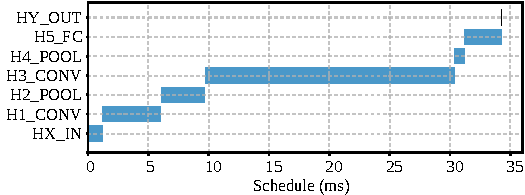
\includegraphics[width=1\columnwidth]{../figures/latency_sw.pdf}
	\caption{Computation on embedded CPU.}
	\label{fig:latency_sw}
\end{figure}

\subsubsection{Benchmark on tensor processor with standard floating-point computation}
To benchmark the computation on hardware TP with standard floating-point, we implement the system architecture with one TP. In this case, the embedded software builds the CNN as a sequential model mapping \emph{Conv2D} tensor operations to the TP at 200 MHz as clock frequency. The hardware mapping and the computation schedule of this deployment are displayed in \Tab{tab:latency_fp} and \fig{fig:latency_pu_fp}.

\begin{table}[!t]\centering
	\caption{Performance of TP with standard floating-point (IEEE 754) computation.}\label{tab:latency_fp}
	\scriptsize
	\begin{tabular}{llrrrrrr}\toprule
		\multicolumn{2}{c}{\textbf{Hardware mapping}} & &\multicolumn{4}{c}{\textbf{Computation schedule (ms)}} \\\cmidrule{1-2}\cmidrule{4-7}
		\textbf{Layer} &\textbf{PU} & &$t_s$ &$t_{CPU}$ &$t_{PU}$ &$t_f$ \\\midrule
		HX\_IN &Spike & &0 &0.056 &0.370 &0.426 \\
		H1\_CONV &Conv1 & &0.058 &0.598 &2.002 &2.658 \\
		\multirow{2}{*}{H2\_POOL}
		&Pool1 & &0.658 &0.126 &1.091 &1.875 \\
		&Pool2 & &0.785 &0.125 &1.075 &1.985 \\
		\multirow{2}{*}{H3\_CONV} 
		&Conv2 & &0.911 &0.280 &3.183 &4.374 \\
		&Conv3 & &1.193 &0.279 &3.176 &4.648 \\
		H4\_POOL &Pool3 & &1.473 &0.037 &0.481 &1.991 \\
		H5\_FC &FC & &1.512 &0.101 &1.118 &2.731 \\
		HY\_OUT &CPU & &1.615 &0.004 &0 &1.619 \\
		\bottomrule
	\end{tabular}
\end{table}

\begin{figure}[!t]
	\centering
	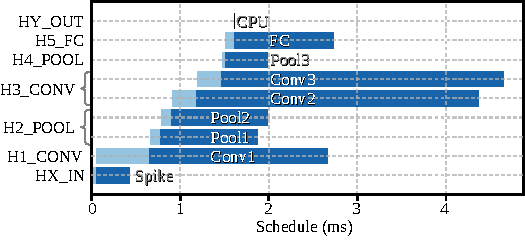
\includegraphics[width=1\columnwidth]{../figures/latency_pu_fp.pdf}
	\caption{Performance of TP with standard floating-point (IEEE 754) computation.}
	\label{fig:latency_pu_fp}
\end{figure}


The post-implementation resource utilization and power dissipation are shown in \Tab{tab:resource_fp}.

The TP instantiates an on-chip weight matrix of \REVIEWR{$52,000$} entries, wish is sufficient to store \REVIEWR{$W\in\mathbb{R}^{5\times 5\times 2\times 32}$} and $B\in\mathbb{R}^{5\times 5\times 32\times 64}$ for weight and bias, respectively. In order to reduce BRAM utilization, we use a custom floating-point representation composed of 4-bit exponent and 4-bit mantissa. Each 8-bit entry is promoted to its standard floating-point representation for computation.

\begin{table}[!h]\centering
	\caption{Resource utilization and power dissipation with standard floating-point (IEEE 754) computation.}\label{tab:resource_fp}
	\scriptsize
	\begin{tabular}{lrrrrrrr}\toprule
		\textbf{PU} & &\textbf{LUT} &\textbf{FF} &\textbf{DSP} &\textbf{BRAM 18K} &\textbf{Power (mW)} \\\midrule
		Spike & &2,640 &4,903 &2 &2 &38 \\
		Conv & &2,765 &4,366 &19 &37 &89 \\
		Pool & &2,273 &3,762 &5 &3 &59 \\
		FC & &2,649 &4,189 &8 &9 &66 \\
		\bottomrule
	\end{tabular}
\end{table}

\REVIEW{The implementation of dot-product with standard floating-point arithmetic (IEEE 754) utilizes proprietary multiplier and adder floating-point operator cores. Vivado HLS accomplishes floating-point arithmetic operations by mapping them onto Xilinx LogiCORE IP cores, these floating-point operator cores are instantiated in the resultant RTL\mbox{\cite{hrica2012floating}}. In this case, the implementation of the dot-product with the standard floating-point computation reuses the multiplier and adder cores already instantiated in other compute sections of the TP. The post-implementation resource utilization and power dissipation of the floating-point operator cores are shown in {\Tab{tab:LogiCORE}}.}

\begin{table}[!h]\centering
	\caption{Resource utilization and power dissipation of multiplier and adder floating-point (IEEE 754) operator cores.}\label{tab:LogiCORE}
	\scriptsize
	\begin{tabular}{lrrrrrr}\toprule
		\textbf{Core operation} &\textbf{DSP} &\textbf{FF} &\textbf{LUT} &\textbf{Latency (clk)} &\textbf{Power (mW)} \\\midrule
		Multiplier &3 &151 &325 &4 &7 \\
		Adder &2 &324 &424 &8 &6 \\
		\bottomrule
	\end{tabular}
\end{table}

\subsection{Design exploration with hybrid custom floating-point and logarithmic approximation}

In this section, we address a design exploration to evaluate our approach for inference using hybrid custom floating-point and logarithmic approximation. First, we examine the weight matrix of each convolution layer in order to determine the minimum requirements for numeric representation and memory storage. Second, we implement the TP using the minimal floating-point and logarithmic representation as design parameters. Finally, we evaluate the overall performance, inference accuracy, resource utilization, and power dissipation.

\subsubsection{Parameters for numeric representation of weight matrix}
\label{sec:parameters}
We obtain information for the numerical representation of the synaptic weight matrices from their $\log_2$-histograms presented in {\fig{fig:log2histogram}}. These histograms show the distribution of weight values in each matrix. We observe that the minimum integer exponent value is \REVIEWR{$-13$}. Hence, applying \REVIEWR{\equ{eq:exp_max}} and \REVIEWR{\equ{eq:bits_exp}} to the given CNN, we obtain \REVIEWR{$E_{\min}=-13$ and $N_E=4$}, respectively. Therefore, 4-bits are required for the absolute binary representation of the exponents.

For quality configurability, the mantissa bit-width is a knob parameter that is tuned by the designer. This procedure leverages the builtin error-tolerance of neural networks and performs a trade-off between resource utilization and QoR. In the following subsection, we present a case study with 1-bit mantissa corresponding to the custom floating-point approximation.

\begin{figure}[t!]
	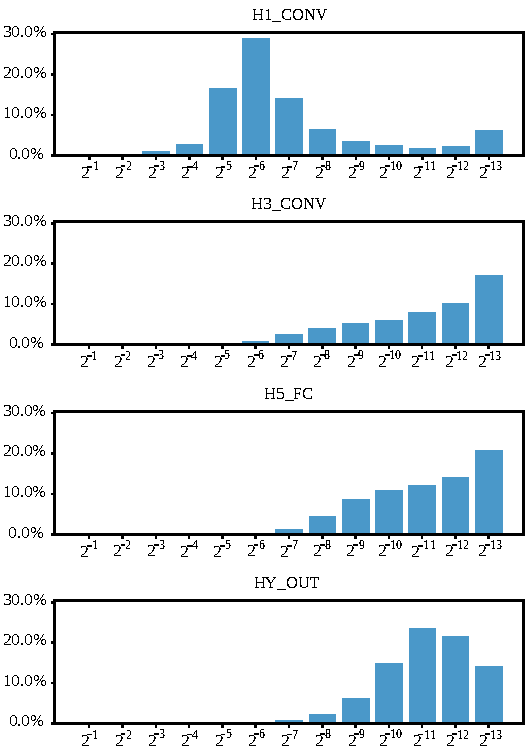
\includegraphics[width=\columnwidth]{../figures/log2_histogram.pdf}
	\caption{$\log_2$-histogram of each synaptic weight matrix showing the percentage of matrix elements with given integer exponent.}\label{fig:log2histogram}
\end{figure}

\subsubsection{Design exploration for dot-product with hybrid custom floating-point approximation}
For this design exploration, we use a custom floating-point representation composed of 4-bit exponent and 1-bit mantissa. This format is used for both the filter matrix and bias vectors of each convolution layer. The TP instantiates on-chip stationary both the filter matrix and bias vectors for \REVIEWR{$X$ and $Y$} entries of 6-bit (S1E4M1). The available memory size is large enough to store \REVIEWR{$W\in\mathbb{R}^{5\times 5\times 2\times 32}$ and $W\in\mathbb{R}^{5\times 5\times 32\times 64}$} for \REVIEWR{$\vec{F}$ and $\vec{b}$}, respectively. The hardware mapping and the computation schedule of this implementation are displayed in \Tab{tab:latency_cfp} and \Fig{fig:latency_pu_cfp_cycle}.

As shown in the computation schedule in \Tab{tab:latency_cfp} and \Fig{fig:latency_pu_cfp_cycle}, this implementation achieves a peak acceleration of \REVIEWR{55x}, and a power efficiency of \REVIEWR{5.5 GFLOP/s/W}. This configuration achieves an accuracy of \REVIEWR{$90.97\%$} correct regressions on the \REVIEWR{500} validation samples. This indicates an accuracy gain of \REVIEWR{$0.33\%$}.

The post-implementation resource utilization and power dissipation are shown in \Tab{tab:resource_cfp}.

\begin{table}[h!]\centering
	\caption{Resource utilization and power dissipation of processing units with hybrid custom floating-point approximation.}\label{tab:resource_cfp}
	\scriptsize
	\begin{tabular}{lrrrrrrr}\toprule
		\textbf{PU} & &\textbf{LUT} &\textbf{FF} &\textbf{DSP} &\textbf{BRAM 18K} &\textbf{Power (mW)} \\\midrule
		Conv & &3,139 &4,850 &19 &25 &82 \\
		FC & &3,265 &5,188 &8 &9 &66 \\
		\bottomrule
	\end{tabular}
\end{table}

\begin{table}[t!]\centering
	\caption{Performance of hardware processing units with hybrid custom floating-point approximation.}\label{tab:latency_cfp}
	\scriptsize
	\begin{tabular}{llrrrrrr}\toprule
		\multicolumn{2}{c}{\textbf{Hardware mapping}} & &\multicolumn{4}{c}{\textbf{Computation schedule (ms)}} \\\cmidrule{1-2}\cmidrule{4-7}
		\textbf{Layer} &\textbf{PU} & &$t_s$ &$t_{CPU}$ &$t_{PU}$ &$t_f$ \\\midrule
		HX\_IN &Spike & &0 &0.055 &0.307 &0.362 \\
		H1\_CONV &Conv1 & &0.057 &0.654 &1.309 &2.020 \\
		\multirow{2}{*}{H2\_POOL} &Pool1 & &0.713 &0.131 &1.098 &1.942 \\
		&Pool2 & &0.845 &0.125 &1.098 &2.068 \\
		\multirow{2}{*}{H3\_CONV} &Conv2 & &0.972 &0.285 &1.199 &2.456 \\
		&Conv3 & &1.258 &0.279 &1.184 &2.721 \\
		H4\_POOL &Pool3 & &1.538 &0.037 &0.484 &2.059 \\
		H5\_FC &FC & &1.577 &0.091 &0.438 &2.106 \\
		HY\_OUT &CPU & &1.669 &0.004 &0 &1.673 \\
		\bottomrule
	\end{tabular}
\end{table}

\begin{figure}[t!]
	\centering
	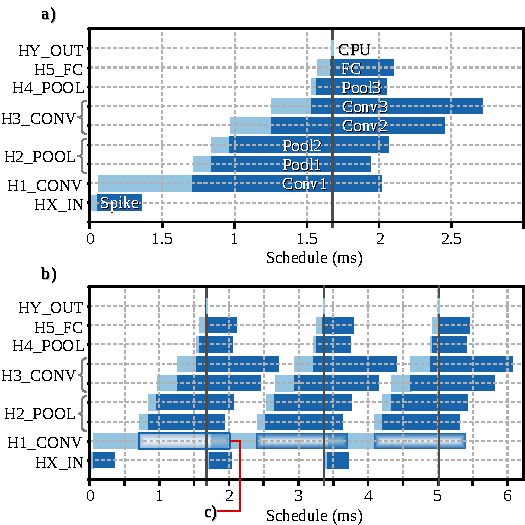
\includegraphics[width=1\columnwidth]{../figures/latency_cfp_cycle.pdf}
	\caption{Performance on processing units with hybrid custom floating-point approximation, (a) exhibits computation schedule, (b) presents cyclic computation schedule, and (c) shows the performance of \emph{Conv2} from a previous computation cycle during the preprocessing of \emph{H1\_CONV} on the current computation cycle without bottleneck.}
	\label{fig:latency_pu_cfp_cycle}
\end{figure}


\subsubsection{Design exploration for dot-product whit hybrid logarithmic approximation}
As the most efficient setup and yet the worst-case quality configuration, we use a 4-bit integer exponent for logarithmic representation of \REVIEWR{$\vec{F}$ and $\vec{b}$}. The hardware mapping and the computation schedule of this implementation are displayed in \Tab{tab:latency_log} and \Fig{fig:latency_pu_log_cycle}. As shown in the computation schedule in \Tab{tab:latency_log} and \Fig{fig:latency_pu_log_cycle}, this implementation achieves a peak acceleration of \REVIEWR{55X} and a power efficiency of \REVIEWR{5.5 GFLOPS/s/W}. This quality configuration achieves an accuracy degradation \REVIEWR{$0.84\%$} on correct regressions on the \REVIEWR{500} validation samples.

The post-implementation resource utilization and power dissipation are shown in \Tab{tab:resource_log}.

\begin{table}[t!]\centering
	\caption{Performance of hardware processing units with hybrid logarithmic approximation.}\label{tab:latency_log}
	\scriptsize
	\begin{tabular}{llrrrrrr}\toprule
		\multicolumn{2}{c}{\textbf{Hardware mapping}} & &\multicolumn{4}{c}{\textbf{Computation schedule (ms)}} \\\cmidrule{1-2}\cmidrule{4-7}
		\textbf{Layer} &\textbf{PU} & &$t_s$ &$t_{CPU}$ &$t_{PU}$ &$t_f$ \\\midrule
		HX\_IN &Spike & &0 &0.055 &0.264 &0.319 \\
		H1\_CONV &Conv1 & &0.057 &0.655 &1.271 &1.983 \\
		\multirow{2}{*}{H2\_POOL} &Pool1 & &0.714 &0.130 &1.074 &1.918 \\
		&Pool2 & &0.845 &0.126 &1.106 &2.077 \\
		\multirow{2}{*}{H3\_CONV} &Conv2 & &0.973 &0.285 &1.179 &2.437 \\
		&Conv3 & &1.258 &0.278 &1.176 &2.712 \\
		H4\_POOL &Pool3 & &1.538 &0.037 &0.488 &2.063 \\
		H5\_FC &FC & &1.577 &0.091 &0.388 &2.056 \\
		HY\_OUT &CPU & &1.669 &0.004 &0 &1.673 \\
		\bottomrule
	\end{tabular}
\end{table}

\begin{figure}[!t]
	\centering
	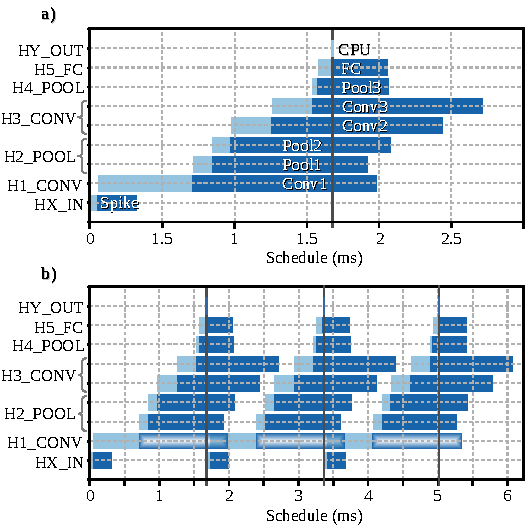
\includegraphics[width=1\columnwidth]{../figures/latency_log_cycle.pdf}
	\caption{Performance of processing units with hybrid logarithmic approximation, (a) exhibits computation schedule, and (b) illustrates cyclic computation schedule.}
	\label{fig:latency_pu_log_cycle}
\end{figure}

\begin{table}[!h]\centering
	\caption{Resource utilization and power dissipation of processing units with hybrid logarithmic approximation.}\label{tab:resource_log}
	\scriptsize
	\begin{tabular}{lrrrrrrr}\toprule
		\textbf{PU} & &\textbf{LUT} &\textbf{FF} &\textbf{DSP} &\textbf{BRAM 18K} &\textbf{Power (mW)} \\\midrule
		Conv & &3,086 &4,804 &19 &21 &78 \\
		FC & &3,046 &4,873 &8 &8 &66 \\
		\bottomrule
	\end{tabular}
\end{table}

\subsection{Results and discussion}
As a reference, the inference on embedded CPU using standard 32-bit floating-point achieves an accuracy gain of \REVIEWR{0.3\%} with a latency of \REVIEWR{3,450.28ms}. As a second reference point, the inference on TP with standard floating-point presents a latency of \REVIEWR{34.5ms}, as result we get a $10.7\times$ latency enhancement.

As a demonstration of the proposed hardware/software architecture, the inference with TP using 5-bit custom floating-point (4-bit exponent, 1-bit mantissa) and 4-bit logarithmic (4-bit exponent) achieves \REVIEWR{$55.5\times$} latency enhancement. This results in an accuracy gain of \REVIEWR{$0.33\%$} and degradation of \REVIEWR{$0.46\%$}, respectively.

Regarding resource utilization and power dissipation, the TP with 5-bit custom floating-point has a \REVIEWR{$43.24\%$} reduction of BRAM, and a \REVIEWR{$12.35\%$} of improvement in energy efficiency over the standard floating-point implementation. \REVIEW{However, the hybrid dot-product with custom floating-point does not reuse the available floating-point operator cores instantiated from other computational sections (see {\Tab{tab:LogiCORE}}). Therefore, the logic required for the dot-product must be implemented, which is reflected as additional utilization of LUT and FF resources.} The experimental results of the design exploration are summarized in \Tab{tab:results}. \REVIEW{The platform implementations are summarized in \mbox{\Tab{tab:platform_comparison}}, and their power dissipation breakdowns are presented in {\fig{fig:platform_power_dissipation_breakdown}}.}

\begin{table*}[!t]
	\begin{threeparttable}
		\centering
		\caption{Experimental results.}\label{tab:results}
		\scriptsize
		\begin{tabular}{lrrrrrrrrrrrrrr}\toprule
			\multirow{2}{*}{\textbf{Dot-product implementation}} &\multirow{2}{*}{\textbf{PU}} &\multicolumn{4}{c}{\textbf{Post-implementation resource utilization}} & &\multirow{2}{*}{\textbf{Power (mW)}} & &\multicolumn{2}{c}{\textbf{Latency}} & &\multicolumn{2}{c}{\textbf{Accuracy (\%)\tnote{e}}} \\\cmidrule{3-6}\cmidrule{10-11}\cmidrule{13-14}
			& &\textbf{LUT} &\textbf{FF} &\textbf{DSP} &\textbf{BRAM 18K} & & & &$T_{SC}$ \textbf{(ms)} &\textbf{Gain\tnote{d}} & &\textbf{Noise 0\%} &\textbf{50\%} \\\midrule
			\multirow{2}{*}{Standard floating-point computation\tnote{a}} &Conv &2,765 &4,366 &19 &37 & &89 & &\multirow{2}{*}{3.18} &\multirow{2}{*}{10.7x} & &\multirow{2}{*}{98.98} &\multirow{2}{*}{98.63} \\
			&FC &2,649 &4,189 &8 &9 & &66 & & & & & & \\
			& & & & & & & & & & & & & \\
			\multirow{2}{*}{Hybrid custom floating-point approx\tnote{b}} &Conv &3,139 &4,850 &19 &25 & &82 & &\multirow{2}{*}{1.67} &\multirow{2}{*}{20.5x} & &\multirow{2}{*}{98.97} &\multirow{2}{*}{98.47} \\
			&FC &3,265 &5,188 &8 &9 & &66 & & & & & & \\
			& & & & & & & & & & & & & \\
			\multirow{2}{*}{Hybrid logarithmic approximation\tnote{c}} &Conv &3,086 &4,804 &19 &21 & &78 & &\multirow{2}{*}{1.67} &\multirow{2}{*}{20.5x} & &\multirow{2}{*}{98.84} &\multirow{2}{*}{95.22} \\
			&FC &3,046 &4,873 &8 &8 & &66 & & & & & & \\
			\bottomrule
		\end{tabular}
		\begin{tablenotes}
			\scriptsize
			\item[a] Reference with standard floating-point arithmetic (IEEE 754).
			\item[b] Synaptic weight with number representation composed of 4-bit exponent and 1-bit mantissa.
			\item[c] Synaptic weight with number representation composed of 4-bit exponent.
			\item[d] Acceleration with respect to the computation on embedded CPU (ARM Cortex-A9 at 666 MHz) with latency $T_{SC} = 34.28 ms$.
			\item[e] Accuracy on 10,000 image test set with 1000 spikes.
		\end{tablenotes}
	\end{threeparttable}
\end{table*}

\begin{table*}[!t]
	\begin{threeparttable}
		\centering
		\caption{Platform implementations.}\label{tab:platform_comparison}
		\scriptsize
		\begin{tabular}{lrrrrrrrrrr}\toprule
			\multirow{2}{*}{\textbf{Platform implementation}} &\multicolumn{4}{c}{\textbf{Post-implementation resource utilization}} &\multirow{2}{*}{\textbf{Power (W)}} &\multirow{2}{*}{\textbf{Clock (MHz)}} &\multicolumn{2}{c}{\textbf{Latency}} &\multirow{2}{*}{\textbf{Accuracy (\%)\tnote{f}}} \\\cmidrule{2-5}\cmidrule{8-9}
			&\textbf{LUT} &\textbf{FF} &\textbf{DSP} &\textbf{BRAM 18K} & & &$T_{SC}$ \textbf{(ms)} &\textbf{Gain\tnote{e}} & \\\midrule
			\Refs{nevarez2020accelerator}\tnote{a} &42,740 &57,118 &49 &92 &2.519 &250 &4.65 &7.4x &99.02 \\
			This work (standard floating-point computation)\tnote{b} &39,514 &56,036 &82 &180 &2.420 &200 &3.18 &10.7x &98.98 \\
			This work (hybrid custom floating-point approx)\tnote{c} &42,021 &58,759 &82 &156 &2.369 &200 &1.67 &20.5x &98.97 \\
			This work (hybrid logarithmic approximation)\tnote{d} &41,060 &57,862 &82 &148 &2.324 &200 &1.67 &20.5x &98.84 \\
			\bottomrule
		\end{tabular}
		\begin{tablenotes}
			\scriptsize
			\item[a] Reference architecture with homogeneous AUs using standard floating-point arithmetic (IEEE 754).
			\item[b] Reference architecture with specialized heterogeneous PUs using standard floating-point arithmetic (IEEE 754).
			\item[c] Proposed architecture with specialized heterogeneous PUs using synaptic weight with number representation composed of 4-bit exponent and 1-bit mantissa.
			\item[d] Proposed architecture with specialized heterogeneous PUs using synaptic weight with number representation composed of 4-bit exponent.
			\item[e] Acceleration with respect to the computation on embedded CPU (ARM Cortex-A9 at 666 MHz) with latency $T_{SC} = 34.28 ms$.
			\item[f] Accuracy on 10,000 image test set with 1000 spikes.
		\end{tablenotes}
	\end{threeparttable}
\end{table*}

\begin{figure*}[!h]
	\centering
	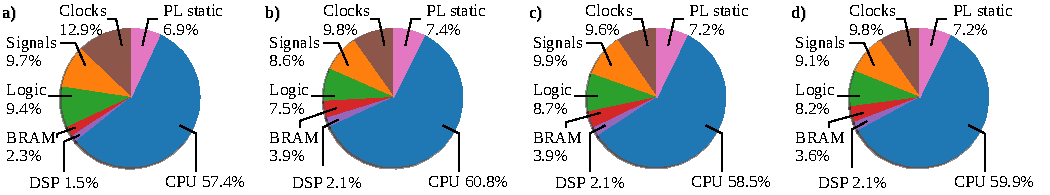
\includegraphics{../figures/platform_power_dissipation_breakdown.pdf}
	\caption{Power dissipation breakdown of platform implementations, (a) \Refs{nevarez2020accelerator} architecture with homogeneous AUs using standard floating-point arithmetic (IEEE 754), (b) reference architecture with specialized heterogeneous PUs using standard floating-point arithmetic (IEEE 754), (c) proposed architecture with hybrid custom floating-point approximation, and (d) proposed architecture with hybrid logarithmic approximation.}
	\label{fig:platform_power_dissipation_breakdown}
\end{figure*}


\subsection{Hardware design exploration}
To evaluate the methodology, we employ \Equ{eq:channel_in_memory}, giving the maximum hyper parameters from models $A$ and $B$: $W_{I}=32$, $C_{I}=60$, $C_{O}=120$, $K_{W} = K_{H} =3$. For the number formats, $BitSize_{I}=32$-b, and $BitSize_{F} = BitSize_{B}=6$-bits. To determine $V_{M}$, we use HLS tool, which gives an estimate of 6 RAM blocks. The performance evaluation and the hardware resource utilization are displayed in \tab{tab:perf} and \tab{tab:resource}, respectively.

\begin{enumerate}
\item{\textbf{XC7Z007S}}: As a resource-limited FPGA, this device has a capacity of 14,400 LUTs and 1.8Mb of BRAM. This limitation allows to instantiate one TP with \emph{Conv} due to its LUT capacity. With \Equ{eq:tp_memory}, we obtain a BRAM utilization of 789.84Kb. This implementation presents a peak runtime acceleration of $55\times$ in model $A$ at the tensor operation \emph{(3A) Conv} with a power reduction of $808\times$.

\item{\textbf{XC7Z010}}: This device has a capacity of 17,600 LUTs and 2.1Mb of BRAM. These resources allow to instantiate two TPs with \emph{Conv}, and one TP with \emph{Conv} and \emph{DConv} engines. With \Equ{eq:tp_memory}, we obtain a BRAM utilization of 1,580Kb. This implementation presents a peak runtime acceleration of $105\times$ in model $A$ at the tensor operation \emph{(3A) Conv} with a power reduction of $1121\times$. On model $B$, \emph{(6B) Conv} presents a peak acceleration of $43.8\times$. The \emph{DConv} tensor operator yields an acceleration of $6.75 \times$, which is limited since the pipelined vector dot-product performs on channel wise.
\end{enumerate}

\begin{table}[!h]\centering
	\caption{Hardware resource utilization and estimated power dissipation.}\label{tab:resource}
	\scriptsize
	\begin{tabular}{lrrrrrrr}\toprule
		\multirow{2}{*}{\textbf{Device}} &\multirow{2}{*}{\textbf{TP}} &\multicolumn{4}{c}{\textbf{Post-implementation resource utilization}} &\multirow{2}{*}{\textbf{Power (W)}} \\\cmidrule{3-6}
		& &\textbf{LUT} &\textbf{FF} &\textbf{DSP} &\textbf{BRAM 36Kb} & \\\midrule
		\multirow{2}{*}{XC7Z007S} &\multirow{2}{*}{1} &7,939 &8,955 &20 &25 &\multirow{2}{*}{1.44} \\
		& &55\% &31\% &30\% &50\% & \\\midrule
		\multirow{2}{*}{XC7Z010} &\multirow{2}{*}{2} &13,542 &15,279 &36 &46 &\multirow{2}{*}{1.880} \\
		& &77\% &43\% &45\% &76\% & \\
		\bottomrule
	\end{tabular}
\end{table}
